\begin{frame}{Mock Galaxy Catalogues}
    
    With merger trees and a galaxy-halo relation, mock galaxy catalogues can be obtained.
    
    Two sets of mock galaxy catalogues were created and tested.
    Both contain $512^3 \approx 1.3 \times 10^8$ particles, but different box sizes were used: \gsmall\ spans $69 Mpc$ in each direction, \glarge\ $100Mpc$.
    The mass resolution for particles corresponds to $9.59\times 10^7 \msol$ and $3.09 \times 10^8\msol$, respectively.
    
    The mass threshold for clumps was chosen to be $10$ particle masses.
    
\end{frame}



\begin{frame}{Testing Mock Galaxy Catalogues}
    
    The performed tests of the mock galaxy catalogues are:
    
    \begin{enumerate}
        \item Stellar Mass Functions $\Phi(M_*)$
        
        give number density of central galaxies with stellar mass $M_*$, directly compared to observational data
        
        \item Clustering Statistics
        
        The two-point correlation function $\xi(r)$ is commonly used as a measure of galaxy clustering.
        It can be interpreted as the excess probability to find a galaxy in a volume element at a separation $r$ from another galaxy compared to what is expected for a uniform random distribution.
    \end{enumerate}
    
\end{frame}



{
    \setbeamertemplate{background}
    {\vbox to \paperheight{\vspace{1.2cm} \hbox to \paperwidth{\hfil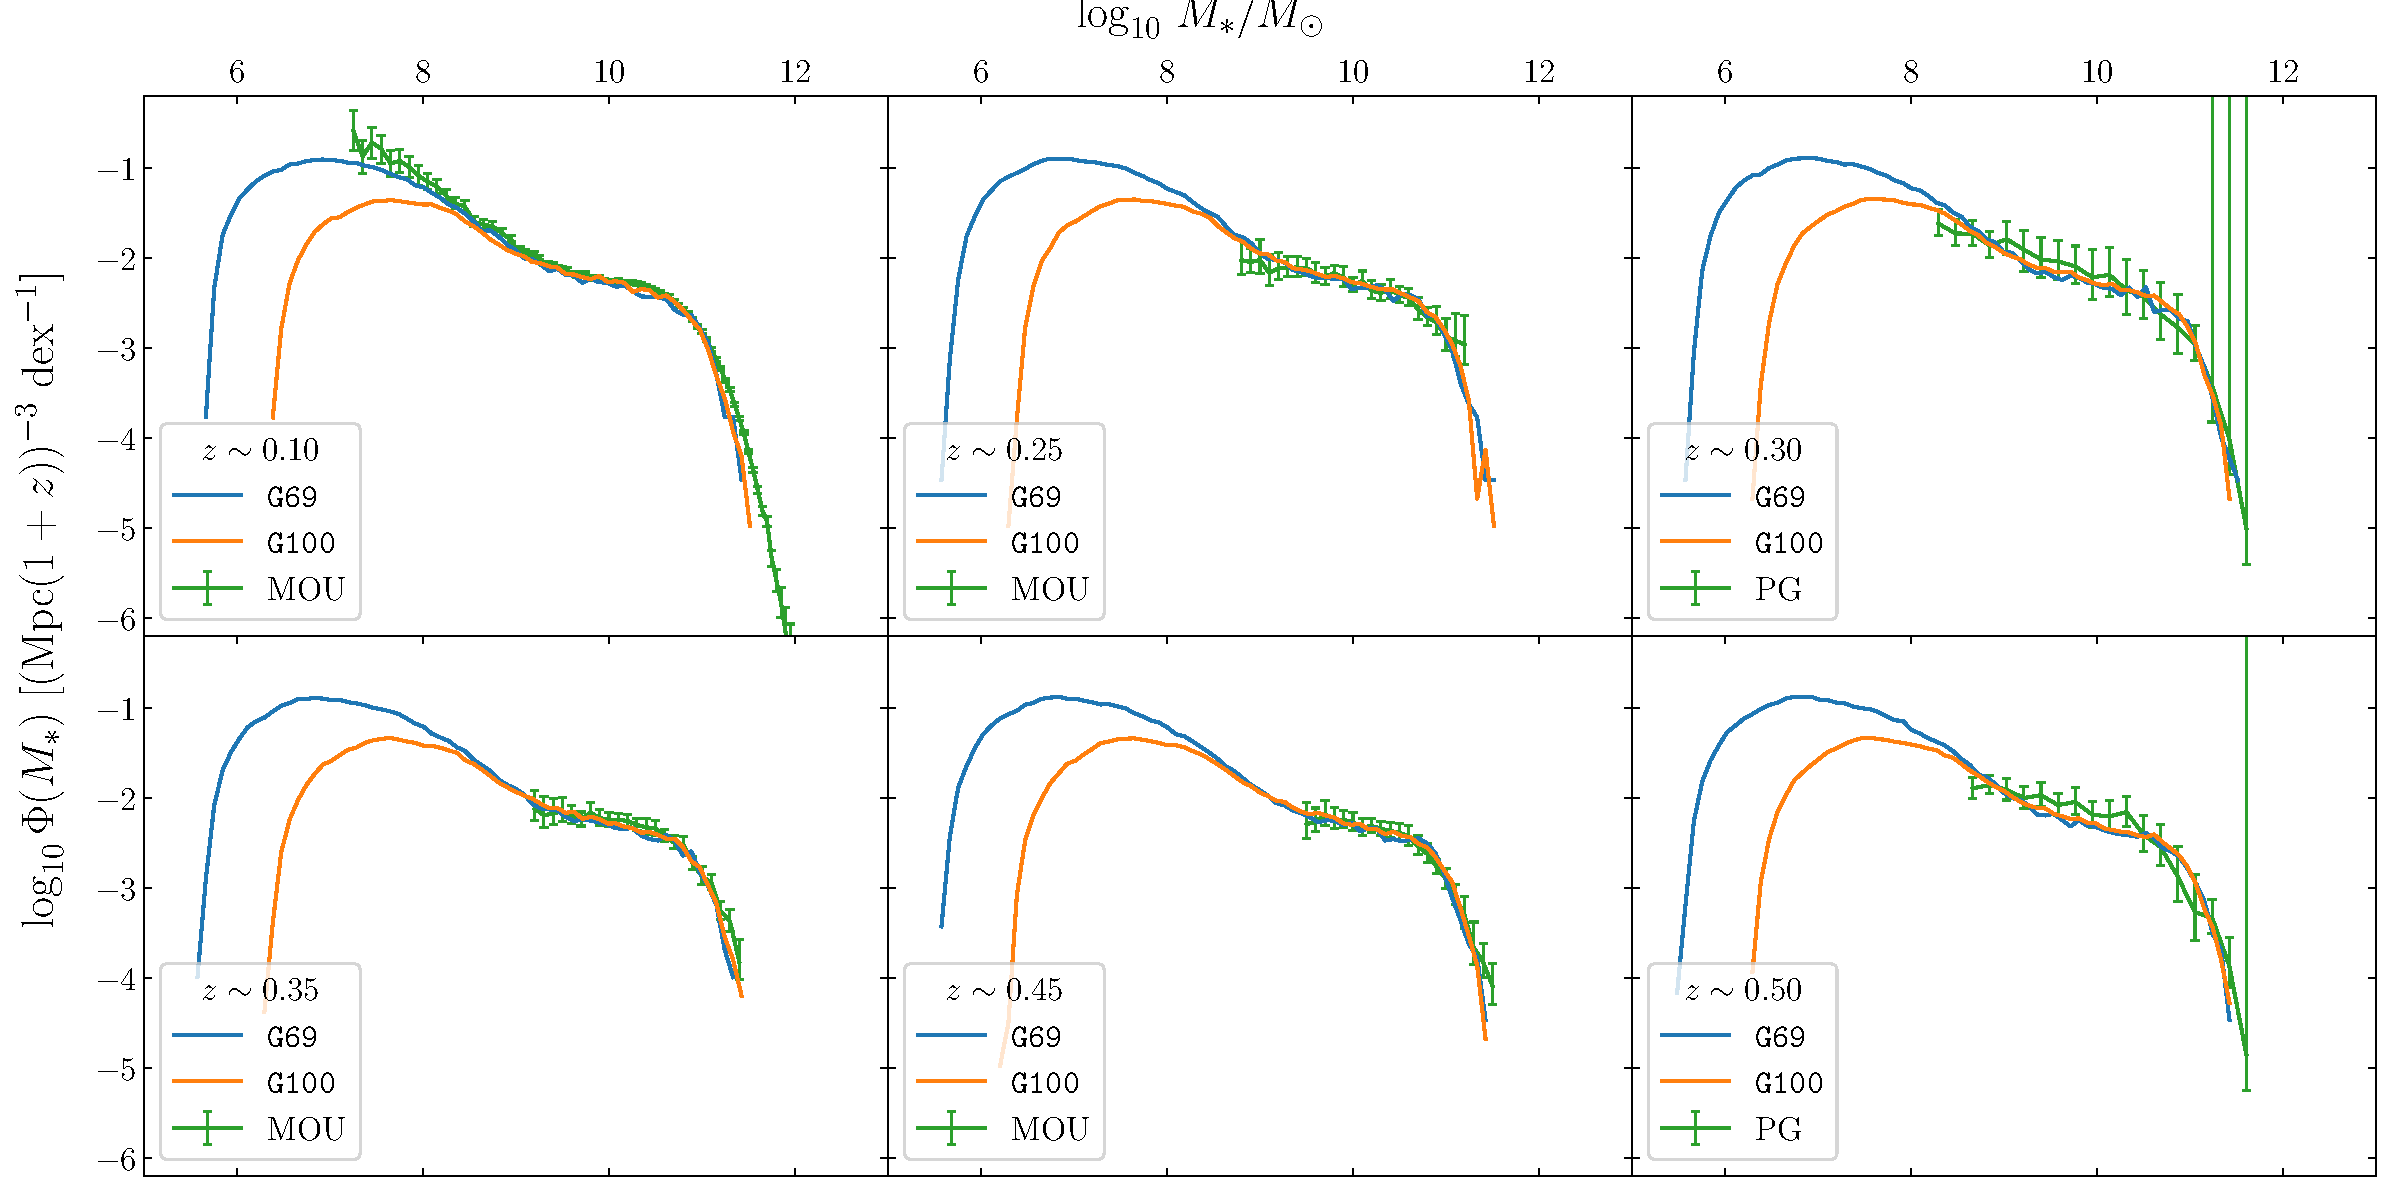
\includegraphics[keepaspectratio,height=\paperheight, width=\paperwidth]{./images/smf/smf_presentation_both_sims-1.pdf}\hfil}\vfil}}
    \begin{frame}
        \frametitle{Stellar Mass Functions: $z=0-0.5$}
        \vspace{6.5cm}
        \tiny\texttt{Obtained stellar mass functions $\Phi(M_*)$ of central galaxies for the two simulation datasets \gsmall\ and \glarge, with boxsizes of $69$ and $100$ Mpc, respectively, compared to observed stellar mass functions.
        }
    \end{frame}
}

{
    \setbeamertemplate{background}
    {\vbox to \paperheight{\vspace{1.2cm} \hbox to \paperwidth{\hfil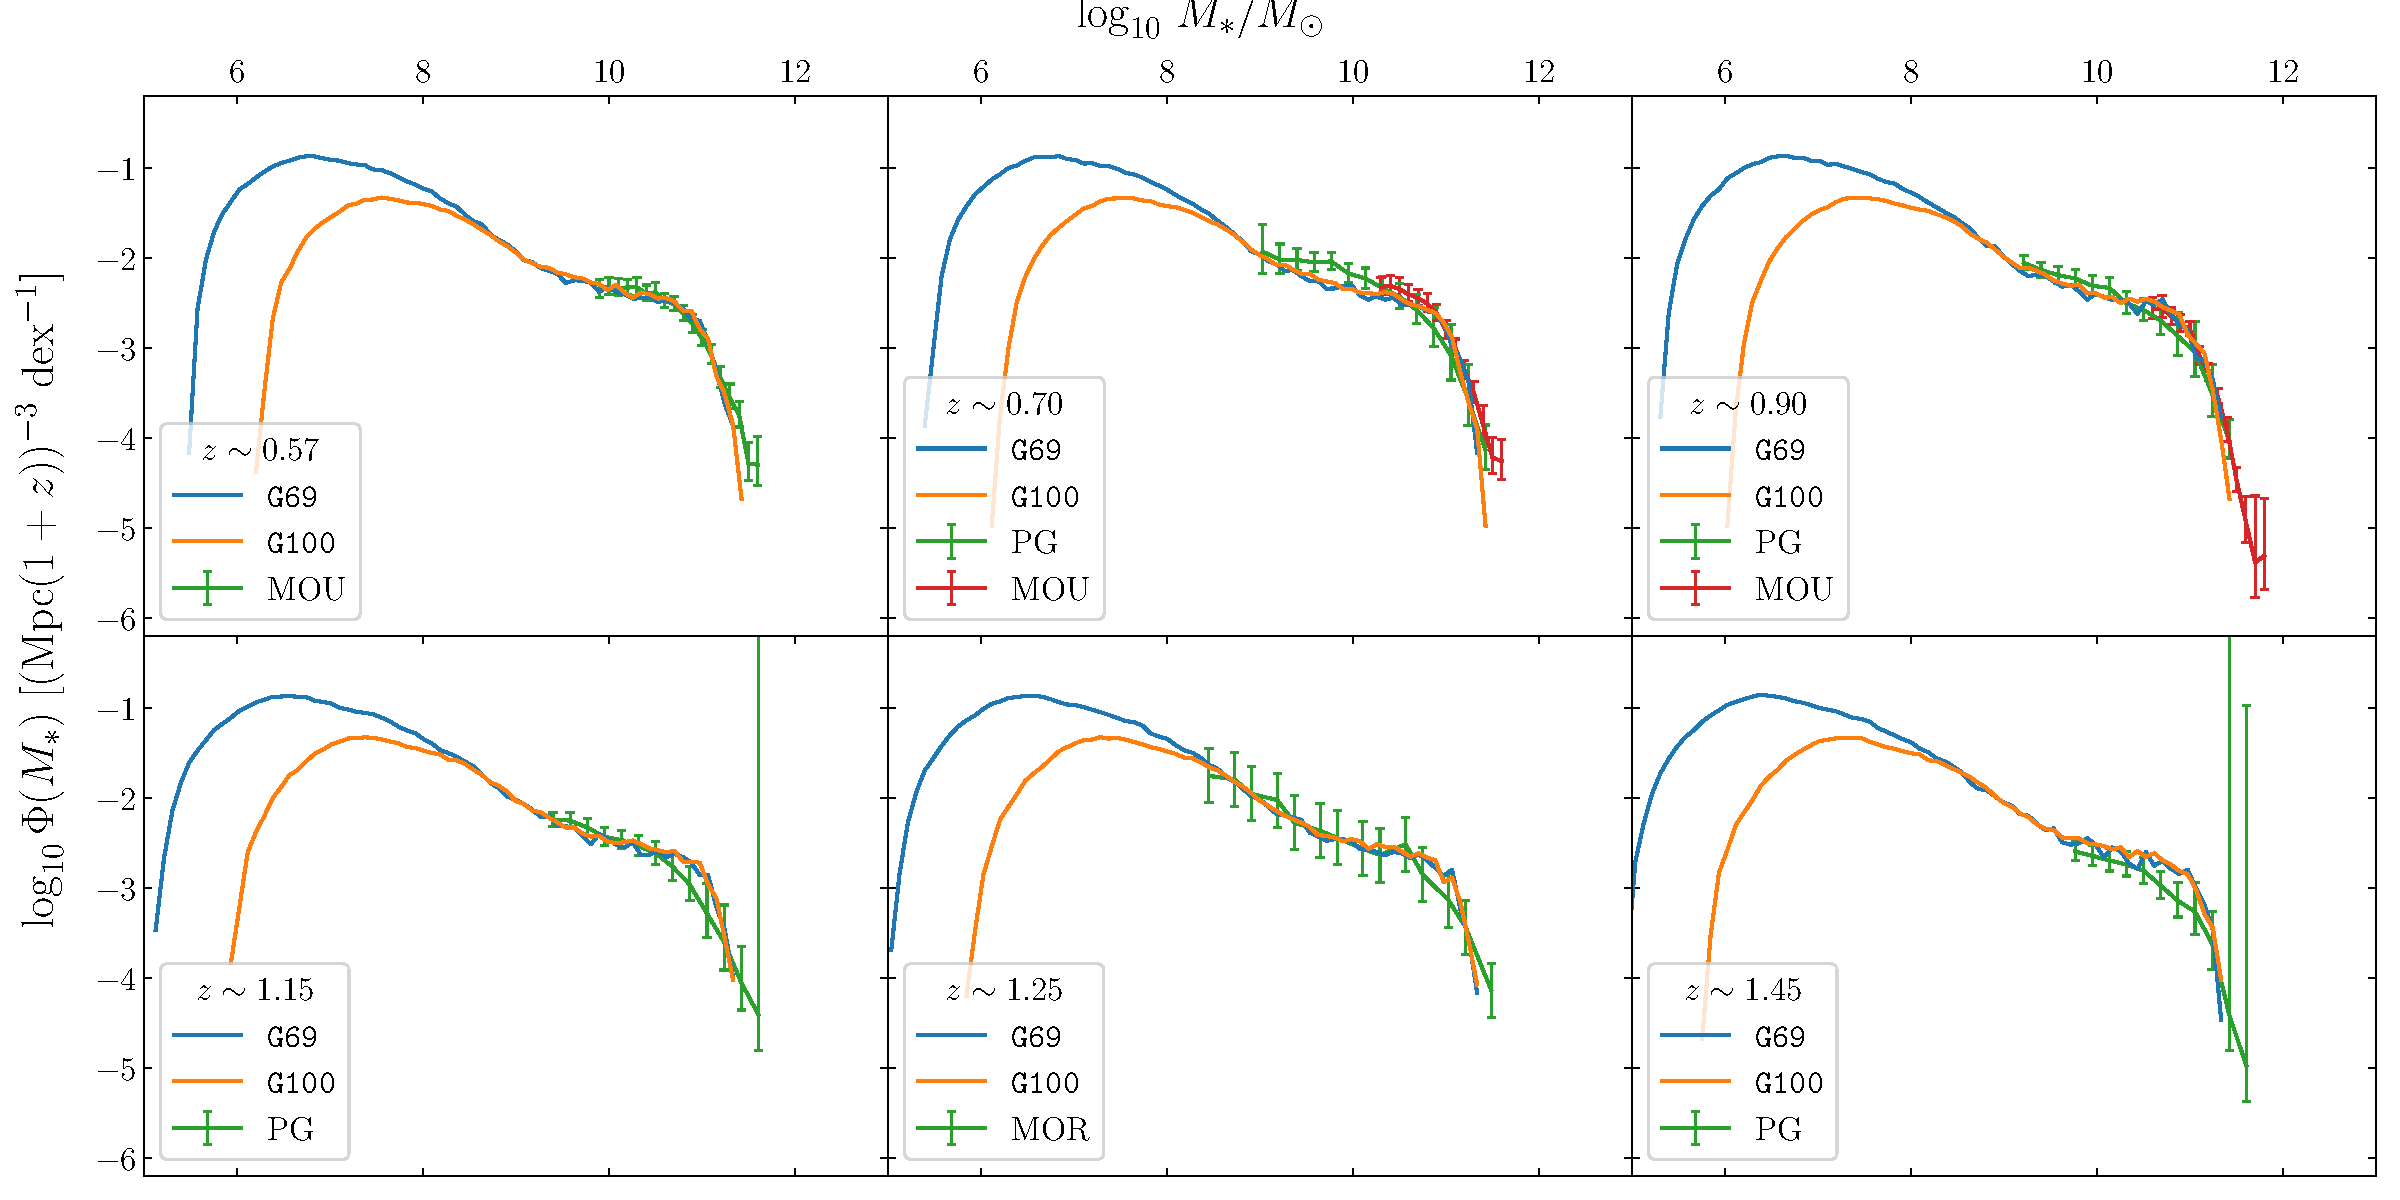
\includegraphics[keepaspectratio,height=\paperheight, width=\paperwidth]{./images/smf/smf_presentation_both_sims-2.pdf}\hfil}\vfil}}
    \begin{frame}
        \frametitle{Stellar Mass Functions: $z=0.5-1.5$}
        \vspace{6.5cm}
        \tiny\texttt{Obtained stellar mass functions $\Phi(M_*)$ of central galaxies for the two simulation datasets \gsmall\ and \glarge, with boxsizes of $69$ and $100$ Mpc, respectively, compared to observed stellar mass functions.
        }
    \end{frame}
}

{
    \setbeamertemplate{background}
    {\vbox to \paperheight{\vspace{1.2cm} \hbox to \paperwidth{\hfil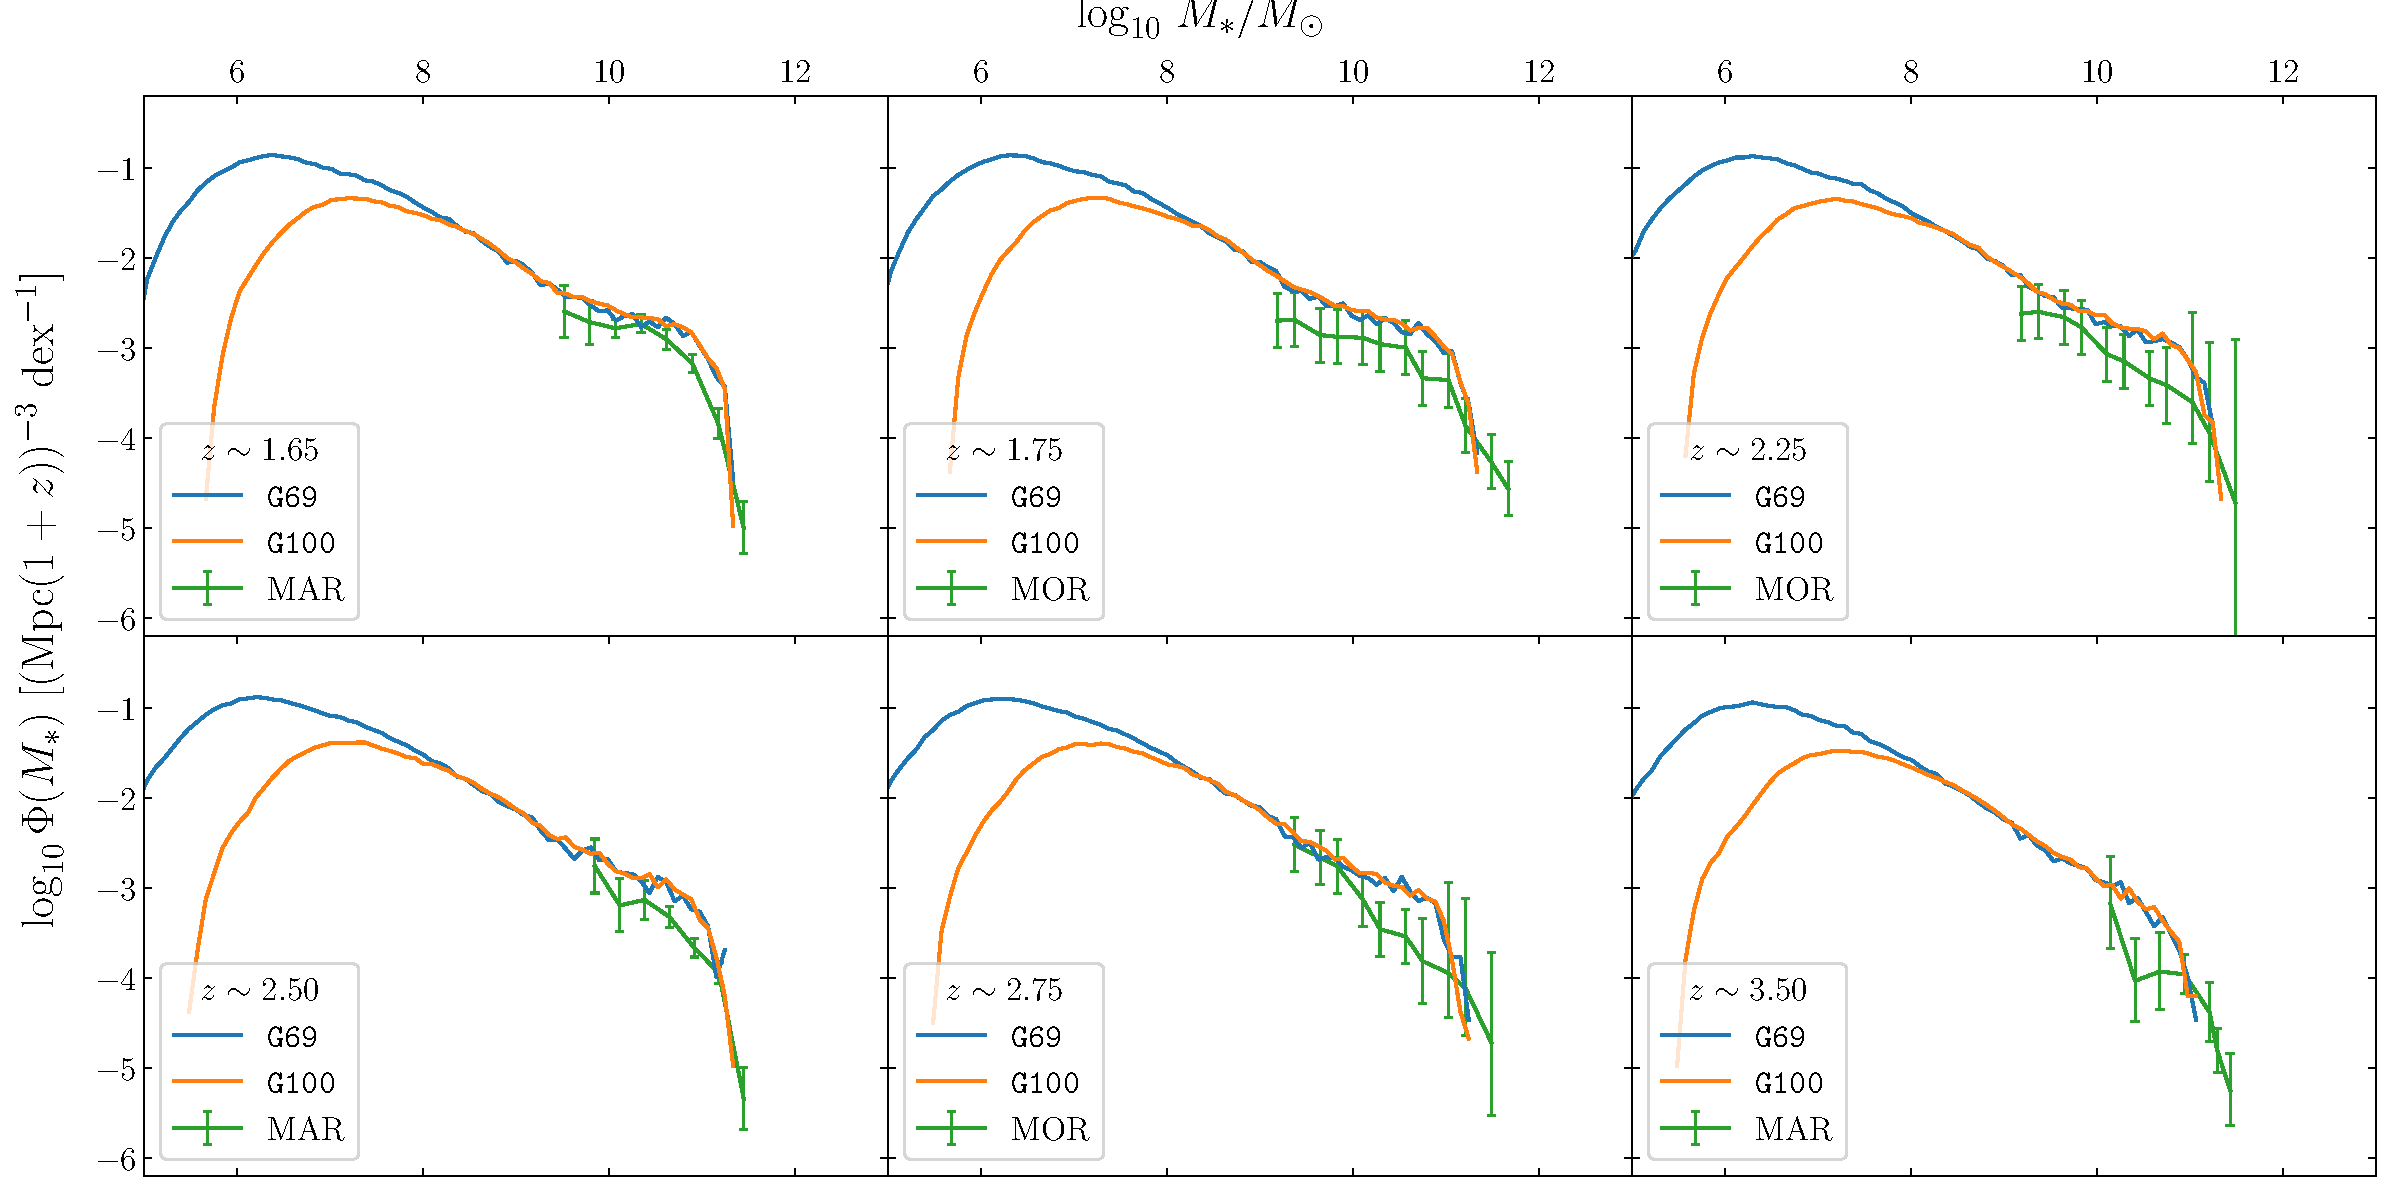
\includegraphics[keepaspectratio,height=\paperheight, width=\paperwidth]{./images/smf/smf_presentation_both_sims-3.pdf}\hfil}\vfil}}
    \begin{frame}
        \frametitle{Stellar Mass Functions: $z=1.5-3.5$}
        \vspace{6.5cm}
        \tiny\texttt{Obtained stellar mass functions $\Phi(M_*)$ of central galaxies for the two simulation datasets \gsmall\ and \glarge, with boxsizes of $69$ and $100$ Mpc, respectively, compared to observed stellar mass functions.
        }
    \end{frame}
}


{
    \setbeamertemplate{background}
    {\vbox to \paperheight{\vspace{1.2cm} \hbox to \paperwidth{\hfil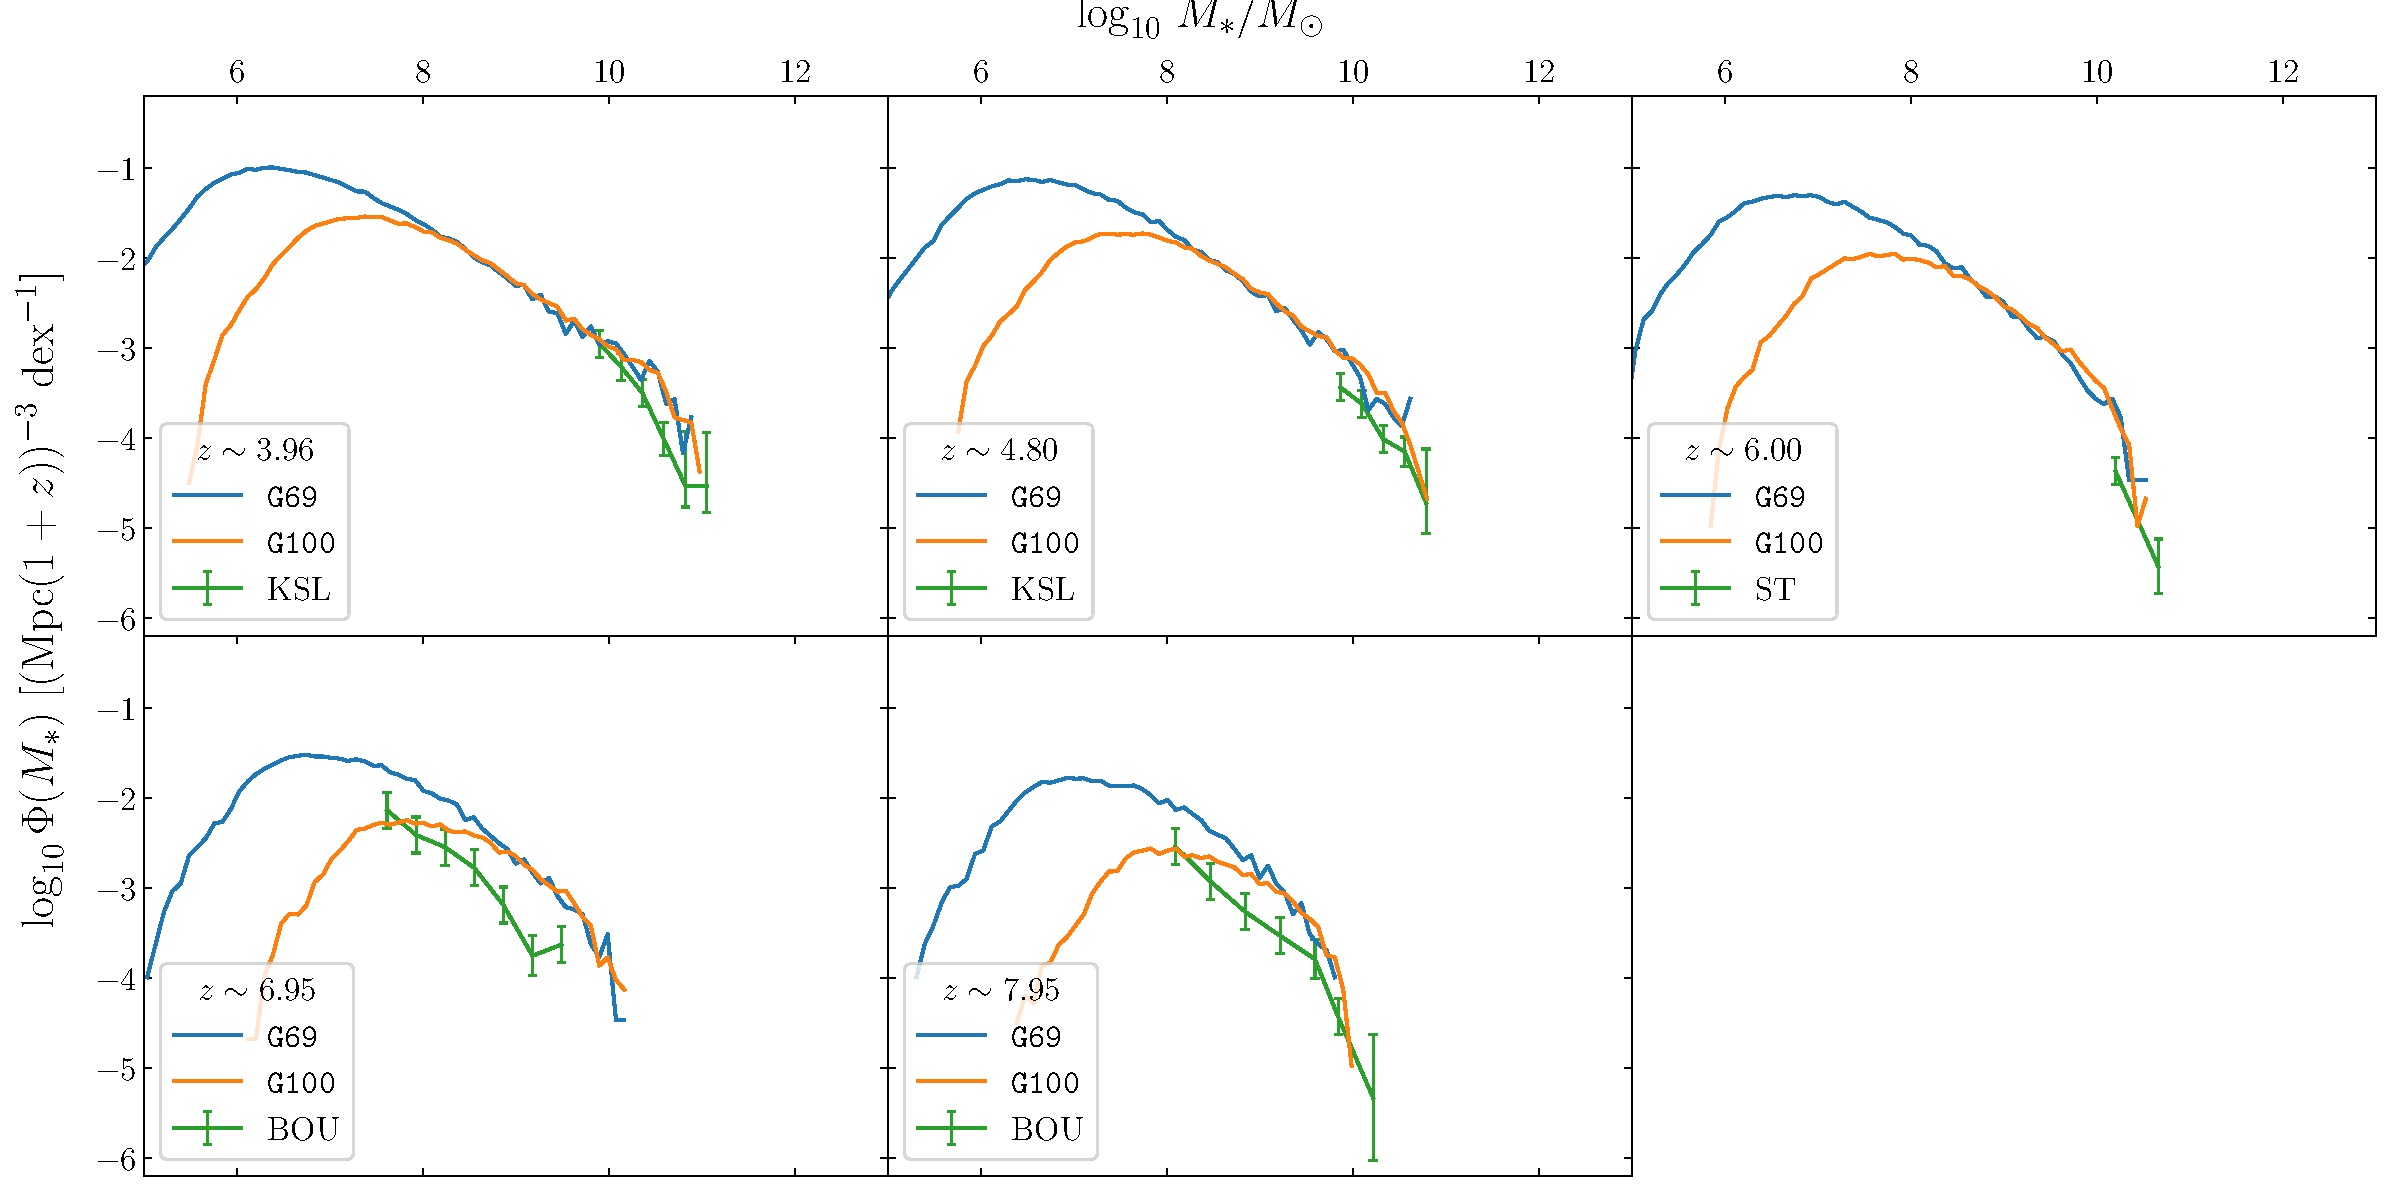
\includegraphics[keepaspectratio,height=\paperheight, width=\paperwidth]{./images/smf/smf_presentation_both_sims-4.pdf}\hfil}\vfil}}
    \begin{frame}
        \frametitle{Stellar Mass Functions: $z=3.5-8$}
        \vspace{6.5cm}
        \tiny\texttt{Obtained stellar mass functions $\Phi(M_*)$ of central galaxies for the two simulation datasets \gsmall\ and \glarge, with boxsizes of $69$ and $100$ Mpc, respectively, compared to observed stellar mass functions.
        }
    \end{frame}
}



%\begin{frame}{Clustering Statistics}
%    Obtaining 2PCF $\xi(r)$:
%    \begin{flalign*}
%    	\delta(\mathbf{r}) &= \frac{\rho(\mathbf{r})}{\langle \rho(\mathbf{r}) \rangle } - 1  && \text{ density contrast} \\
%        \delta_\mathbf{k} &= \frac{1}{V}\int e^{i\mathbf{kr}} \delta(\mathbf{r}) \de ^3 \mathbf{r} && \text{$V = L^3$ periodical volume} \\
%       	P(k)    &= V \langle |\delta_\mathbf{k}|^2 \rangle && \text{Power Spectrum}\\
%        \xi(r)  &= \frac{1}{(2\pi)^3} \int e^{-i\mathbf{kr}} P(k) \de^3 \mathbf{k} && \text{2PCF} \\[.5em]
%       	w_p(r_p) &= 2 \int\limits_{0}^{\infty} \de r_{||} \xi\left( \sqrt{r_{||}^2 + r_{p}^2} \right) && \text{Projected Correlation function}\\
%        &= 2 \int\limits_{r_p}^{\infty} \de r \frac{ r \xi\left( r \right) } {\sqrt{r^2 - r_{p}^2}} && 
%    \end{flalign*}
%        
%\end{frame}
%


{
    \setbeamertemplate{background}
    {\vbox to \paperheight{\vspace{1cm} \hbox to \paperwidth{\hfil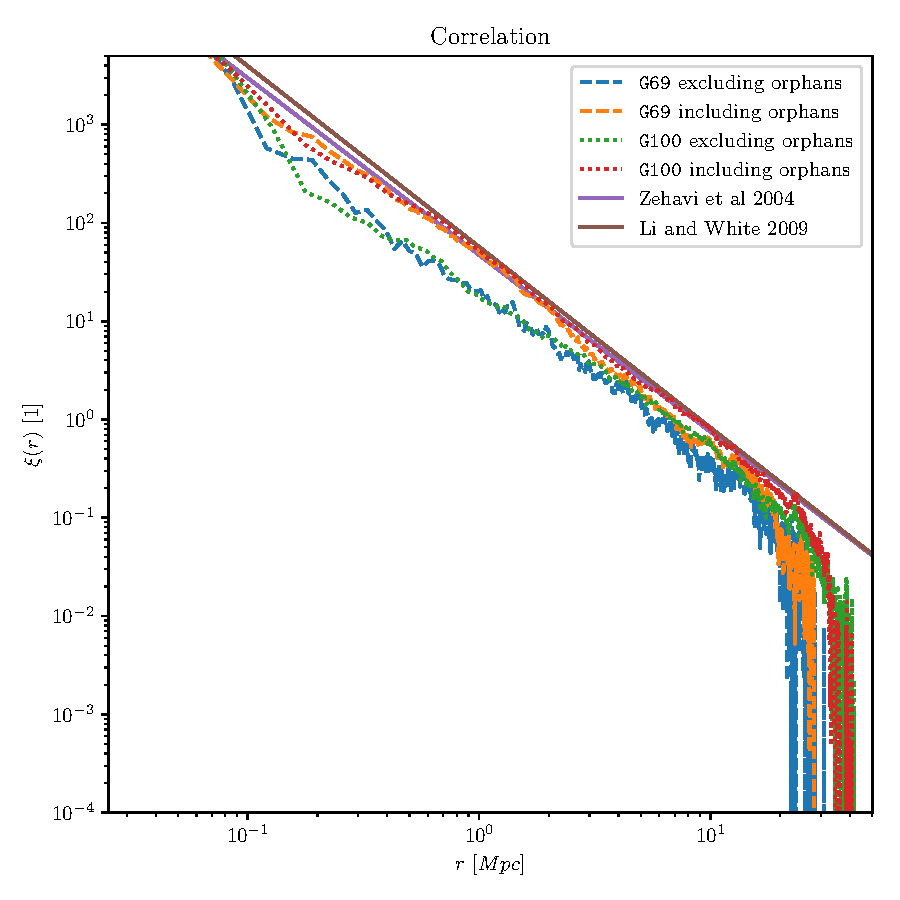
\includegraphics[keepaspectratio,height=.7\paperheight, width=\paperwidth]{./images/correlations/presentation-correlations.pdf}\hfil}\vfil}}
    \begin{frame}
        \frametitle{Correlation Functions}
        \vspace{6.5cm}
        \tiny\texttt{The obtained 2PCF $\xi(r)$ for the \gsmall\ (dashed lines) and \glarge\ (dotted lines) simulations, both including and excluding orphan galaxies, compared to best power law fits of the 2PCF from \cite{LiWhite} and \cite{Correlation1} (solid lines).
        }
    \end{frame}
}


\begin{frame}{Outlook}
    The results show good agreement with observational data, and should improve with increased resolution.
    
    Currently missing: A merging mechanism for individual orphan galaxies. Options would be:
    \begin{itemize}
        \item Introduce some galaxy-galaxy merging cross section
        \item Estimate expected merging time for each orphan galaxy individually, e.g. dynamical friction time or fitted merger timescale by \cite{merger_timescales}
    \end{itemize}
\end{frame}



